%\documentclass{beamer}
\documentclass[handout]{beamer}
\usepackage{amsmath}
\usepackage{amssymb}
\usepackage{tikz}
%\usetikzlibrary{bayesnet}

\title[]{Correctness of Local Probability Propagation\\in Graphical Models with Loops}
\subtitle{by\\Yair Weiss}
\author{Ben Eyal}

\usetheme{Darmstadt}
\usefonttheme{professionalfonts}

\AtBeginSubsection[]
{
    \begin{frame}<beamer>{Outline}
        \tableofcontents[currentsection,currentsubsection]
    \end{frame}
}

\begin{document}

\begin{frame}
    \titlepage
\end{frame}

\begin{frame}{Outline}
    \tableofcontents
\end{frame}

%\section{Thoughts}
%\begin{frame}
%    \begin{enumerate}
%        \item bayesian networks with no loops converge to correct posterior probability
%        \item empirical studies show that bayes nets with loops also converge
%        \item we don't know why it works in theory
%        \item certain single-looped bayes nets can provably be shown to converge
%        \item graphical model - lauritzen 1996
%        \item bayesian network, markov network
%        \item singly-connected networks - belief propagation, pearl 1988
%        \item BU - Belief Update, BR - Belief Revision, MM - Maximum Marginal, MAP - Maximum a Posteriori
%        \item explanation + example of belief update and belief revision on singly-connected markov net
%    \end{enumerate}
%\end{frame}
\section{Introduction}
\subsection{Probability Refresher}
\begin{frame}{Reminder}
    \begin{block}{Conditional Probability}
        \[ \Pr \left( A \mid B \right) = \frac{\Pr \left( A, B \right)}{\Pr \left( B \right)} \]
    \end{block}
    \begin{block}{Bayes' Theorem}
        Bayes' theorem gives us the relation between the posterior probability, $ \Pr \left( A \mid B \right) $, and the prior probability, $ \Pr \left( A \right) $.
        \[ \Pr \left( A \mid B \right) = \frac{\Pr \left( B \mid A \right) \Pr \left( A \right)}{\Pr \left( B \right)} \]
    \end{block}
\end{frame}
\subsection{Definitions}
\begin{frame}
    \begin{itemize}
        \item Correctness
        \item Local Probability Propagation
        \item \alert<2>{Graphical Models}
        \item Loops
    \end{itemize}
\end{frame}
\begin{frame}{Probabilistic Graphical Models}
    \pause
    \begin{definition}
        A Probabilistic Graphical Model (PGM) is a graph, either directed or undirected, in which the nodes correspond to random variables,
        and the edges correspond to direct probabilistic interactions between them.
    \end{definition}
    \begin{block}{Agenda}
        \pause
        In this talk, we'll see how to use PGMs for the task of probabilistic inference.
    \end{block}
\end{frame}
\begin{frame}{Probabilistic Graphical Models}
    \pause
    \begin{definition}
        A Bayes network is a directed acyclic PGM whose edges can be seen as ``cause'' and ``effect'', e.g. an
        edge $ X \rightarrow Y $ means that $ X $ directly influences $ Y $, or ``$ X $ is the cause of $ Y $''.
    \end{definition}
    \pause
    \begin{center}
        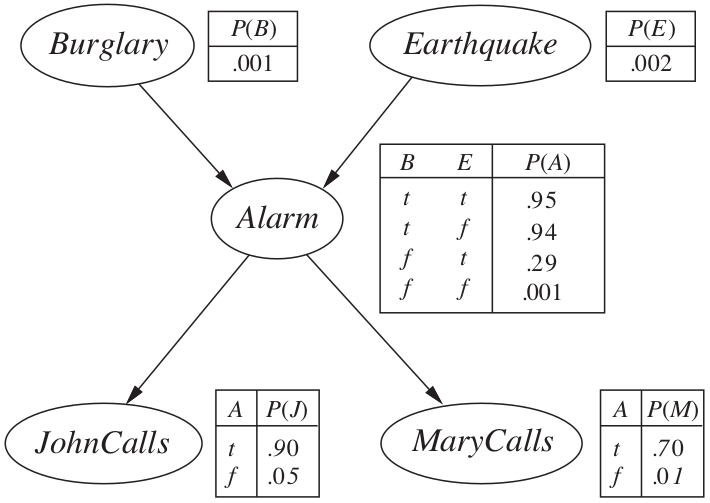
\includegraphics[scale=0.25]{bayesnet}
    \end{center}
\end{frame}
\begin{frame}{Probabilistic Graphical Models}
    \pause
    \begin{definition}
        A Markov Random Field (MRF), or a Markov network, is an undirected PGM which is used when the relations between
        random variables are symmetric, rather than hierarchical, e.g. pixels in an image.
    \end{definition}
    \pause
    \begin{columns}
        \begin{column}[t]{0.2 \textwidth}
            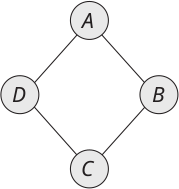
\includegraphics[scale=0.4]{mrf1}
        \end{column}
        \begin{column}[t]{0.8 \textwidth}
            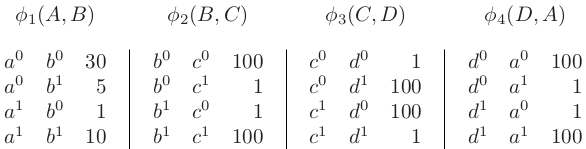
\includegraphics[scale=0.4]{mrf2}
        \end{column}
    \end{columns}
\end{frame}
\begin{frame}
    \begin{itemize}
        \item Correctness
        \item \alert<2>{Local Probability Propagation}
        \item \alert<1>{Graphical Models}
        \item Loops
    \end{itemize}
\end{frame}
\begin{frame}{Belief Propagation}
    content...
\end{frame}
\subsection{The Problem}
\begin{frame}{Belief Propagation}
    content...
\end{frame}
\begin{frame}{``Loopy'' Belief Propagation}
    content...
\end{frame}
\begin{frame}
    \begin{itemize}
        \item How far is the steady-state belief from the correct posterior when the update rules (equations 2.7-2.8) are applied in a loopy network?
        \item What are the conditions under which the BU assignment equals the MM assignment when the update rules are applied in a loopy network?
        \item What are the conditions under which the BR assignment equals the MAP assignment when the update rules are applied in a loopy network?
    \end{itemize}
\end{frame}
\section{Content}
\begin{frame}
\end{frame}
\section{Conclusion}
\begin{frame}
\end{frame}

\end{document}
